%%%%%%%%%%%%%%%%%%%%%%%%%%%%%%%%%%%%%%%%%%%%%%%%%%%%%%%%%%%%%%%%%%%%%%%%%%%%%%%%%%%%%%%%%%%%%%%%%%%%%%%%%%%%%%%%%%%%%%%%

\documentclass{llncs}

%%%%%%%%%%%%%%%%%%%%%%%%%%%%%%%%%%%%%%%%%%%%%%%%%%%%%%%%%%%%%%%%%%%%%%%%%%%%%%%%%%%%%%%%%%%%%%%%%%%%%%%%%%%%%%%%%%%%%%%%
\usepackage{calc}
\usepackage{showframe}

\usepackage[lighttt]{lmodern}

\usepackage[british]{babel}%

\usepackage{subcaption}
\captionsetup{compatibility=false}%

\usepackage{cleveref}%
\usepackage[numbers]{natbib}

\usepackage{listings}

\newlength\listinglinewidth
\setlength\listinglinewidth\linewidth
\addtolength\listinglinewidth{-0.5cm}

\lstset{language=python}
\lstset{lineskip=-4pt}
\lstset{linewidth=\listinglinewidth}
\lstset{xleftmargin=0.25cm}
\lstset{basewidth=0.5em}
\lstset{basicstyle=\ttfamily\footnotesize}
\lstset{keywordstyle=\ttfamily\bfseries}
\lstset{frame=single}

\usepackage{pgf}

% disable with the [disable] option, which will get rid of all of the todos in
% the document! Alternatively, pass 'final' as an option to the document class.
\usepackage[textsize=scriptsize,disable,obeyFinal]{todonotes}

\newcommand{\picalc}{\(\pi\)-calculus }

\hyphenation{}

%%%%%%%%%%%%%%%%%%%%%%%%%%%%%%%%%%%%%%%%%%%%%%%%%%%%%%%%%%%%%%%%%%%%%%%%%%%%%%%%%%%%%%%%%%%%%%%%%%%%%%%%%%%%%%%%%%%%%%%%

\title{Modelling Realistic User Behaviour in Information Systems Simulation Models as Fuzzing Aspects}

\titlerunning{}

\author{Tom Wallis\orcidID{} \and Tim Storer\orcidID{}}

\authorrunning{Wallis and Storer}

\institute{University of Glasgow, Glasgow, Scotland,\\
  \email{w.wallis.1@research.gla.ac.uk},\\
  \email{timothy.storer@glasgow.ac.uk},
}

%%%%%%%%%%%%%%%%%%%%%%%%%%%%%%%%%%%%%%%%%%%%%%%%%%%%%%%%%%%%%%%%%%%%%%%%%%%%%%%%%%%%%%%%%%%%%%%%%%%%%%%%%%%%%%%%%%%%%%%%

\begin{document}

%%%%%%%%%%%%%%%%%%%%%%%%%%%%%%%%%%%%%%%%%%%%%%%%%%%%%%%%%%%%%%%%%%%%%%%%%%%%%%%%%%%%%%%%%%%%%%%%%%%%%%%%%%%%%%%%%%%%%%%%

\maketitle

%%%%%%%%%%%%%%%%%%%%%%%%%%%%%%%%%%%%%%%%%%%%%%%%%%%%%%%%%%%%%%%%%%%%%%%%%%%%%%%%%%%%%%%%%%%%%%%%%%%%%%%%%%%%%%%%%%%%%%%%

\begin{abstract}
  \todo{Spell check for consistency.}

  In this paper we contend that the engineering of information systems is hampered by a paucity of tools to tractably
  model simulate and predict the impact of \emph{realistic} user behaviours on the emergent properties of the overall
  \emph{socio-technical} system, evidenced by the plethora of case studies of system failure in the literature.  We
  address this gap by presenting a novel approach that models ideal user behaviour as workflows and the deviations that
  may arise separately as model fuzzing aspects.  We demonstrate the efficacy of this approach through a case study of
  software development workflows, showing that the application of models of realistic user behaviour to idealised
  workflows results in system behaviour which better simulates that found in the empirical literature.

\end{abstract}

%%%%%%%%%%%%%%%%%%%%%%%%%%%%%%%%%%%%%%%%%%%%%%%%%%%%%%%%%%%%%%%%%%%%%%%%%%%%%%%%%%%%%%%%%%%%%%%%%%%%%%%%%%%%%%%%%%%%%%%%

\section{Introduction}
\label{sec:introduction}

%%%%%%%%%%%%%%%%%%%%%%%%%%%%%%%%%%%%%%%%%%%%%%%%%%%%%%%%%%%%%%%%%%%%%%%%%%%%%%%%%%%%%%%%%%%%%%%%%%%%%%%%%%%%%%%%%%%%%%%%

Information systems are operated within a wider organisational context, characterised by the needs, demands and
behaviours of individual users, interpersonal relationships, organisational structures, business processes, legal or
regulatory standards, and cultural norms \citep{bade07structures,pentland05organisational}.  The
influence of this \emph{socio-technical} interplay on system behaviour (and often failure) has been described in
multiple and diverse case studies of information systems.  Examples of case studies describing socio-technical system
failures include automated emergency vehicle dispatch \citep{robinson96limited}, electronic voting
\citep{lock07observations} and stock market trading systems \citep{cftc-sec10findings}. In each case, system failure
cannot be attributed to either purely user behaviour or information system failure, but instead to an interplay between
both factors within the overall socio-technical system.

Our contention is that these failures arise because systems engineers lack the tools and methods to efficiently model
and accurately simulate the interaction between the information systems and their organisational context, which comprise
a socio- technical system. Without these facilities, systems engineers cannot predict potential socio-technical system
behaviour, during information system design. Simulating this interaction between the information system and users is
hard because user behaviour is heterogeneous, contingent and evolutionary, leading to deviations from idealised
workflows.  Different users have different abilities, training and experiences and can experience phenomena such as
distraction, misjudgments, exhaustion and confusion that can have significant influence on how and when a user completes
a task.  For example, a novice developer working within a large team may be unaware of software development best
practices described in a workflow, perhaps forgetting to make frequent commits to a version control server.  Conversely,
an experienced developer may omit steps, such as peer reviews of their code, they consider unnecessary to optimise their
performance.

Information system users may also adapt their behaviour due to contingencies that arise due to faults in the information
system, the behaviour of other users or the environment \citep{sommerville09deriving}.  In our example scenario, a
software development team may begin reducing quality assurance efforts as a deadline for a release approaches, in an
effort to ensure all required features are completed \citep{beck02test}. Behavior is also continually evolving, as the
autonomous actors in a system adapt to new circumstances, discover optimizations to their workflows, adapt the workflow
to suit local organizational priorities or take shortcuts \citep{bonen79evolutionary}.  In the example scenario, it is
reasonable to anticipate that a novice developer's behaviour will gradually evolve into that of an expert as they gain
more experience.  As a consequence, the de facto behavior exhibited within a system may differ from that envisaged by
system architects in idealized workflows.

A system architect must model their workflows as they are intended to be executed in practice, yet due to their
organisational context any socio-technical system exhibits contingent behaviour which is fundamental to their accurate
simulation. Conventional systems engineering notations for describing user behaviour, such as BPMN \citep{omg2011omgbpmn},
activity diagrams \citep{omg07omguml} and YAWL \citep{hofstede2010yawl} lack features for efficiently modelling these
characteristics.  Attempting to model the heterogeneity, contingency and evolution of user behaviour using these
approaches inevitably results in models that are either too abstract or narrow to be informative, or too complex to be
tractable.  Alternative approaches that abstract the complexity of user behaviour, such as i* \citep{yu1995social},
Kaos \citep{werneck2009goreistarkaos} and Responsibility Modelling \citep{sommerville09deriving} lack sufficient detail to
generate executable simulations.

The key insight of this paper is that the same deviation in behaviour often affects a number of possible actions.
Conversely, a given user's behaviour is the combination of their expected ideal behaviour and the set of deviations that
affect how that user exhibits their behaviour.  Therefore, \emph{we propose and demonstrate the separate
modelling of behavioural irregularities from workflows themselves, showing that they are cross-cutting concerns which can
be applied to an idealised workflow model}.

The two contributions of this paper are as follows:

\begin{itemize}

\item A method for simulating user interactions with information systems that allows for the separate modelling of
  idealised descriptions of workflow and the effects of deviations from those workflows.  We implement our approach in
  an fuzzing aspects software framework, using a combination of aspect oriented programming \cite{filman01aspect} and
  dynamic code fuzzing \citep{takanen08fuzzing}, allowing us to alter the flow of execution in a workflow description
  without sacrificing readability or simplicity.

\item A demonstration of the efficacy of the approach in a case study comparison of Test Driven Development (TDD) and
  Waterfall software development workflows.  The case study demonstates that models of idealised behaviour in software
  development do not conform with the empirical evidence which suggests that TDD out performs Waterfall
  \citep{Bhat2006TestDrivenDevelopment,George2004TestDrivenDevelopment,Huang2009EmpiricalTestFirstProgramming}, but that
  models which incorporate realistic user behaviour when interacting with information systems do.

\end{itemize}

The rest of this paper is structured as follows.  Section \ref{sec:related} discusses related work, covering existing
techniques for modeling socio-technical workflows and the limitations encountered in the literature.  Section
\ref{sec:case-study} introduces the case study problem domain selected to evaluate our approach, and presents the method
for constructing models of socio-technical systems and associated workflows. Section \ref{sec:fuzzing} describes the
development of aspect oriented fuzzing of user behaviour described as workflow models, and the software tool developed
for this purpose.  Section \ref{sec:evaluation} presents our evaluation of the case study and Section
\ref{sec:conclusions} discusses conclusions and future work, as well as noting the potential for applying fuzzing to
other forms of socio-technical models.

%%%%%%%%%%%%%%%%%%%%%%%%%%%%%%%%%%%%%%%%%%%%%%%%%%%%%%%%%%%%%%%%%%%%%%%%%%%%%%%%%%%%%%%%%%%%%%%%%%%%%%%%%%%%%%%%%%%%%%%%

\section{Related Work}
\label{sec:related}

%%%%%%%%%%%%%%%%%%%%%%%%%%%%%%%%%%%%%%%%%%%%%%%%%%%%%%%%%%%%%%%%%%%%%%%%%%%%%%%%%%%%%%%%%%%%%%%%%%%%%%%%%%%%%%%%%%%%%%%%

This section presents a literature review of approaches to modelling the interaction between users and information
systems.  Graphical notations have received considerable attention, perhaps due to their perceived efficacy in
communicating specifications between users, customers and system architects.  Workflow description languages, such as as
UML activity diagrams \citep{omg07omguml}, BPMN \citep{omg2011omgbpmn} and YAWL \citep{hofstede2010yawl} can be used to
denote workflows as directed graphs composed of activities.  Various formalisms are used to underpin these notations and
support analysis.  For example, UML activity diagrams are based on Petri Nets, as is BPMN, but with a richer notation
for expressing more complex aspects of activities, such as differentiating between tasks, activities and transactions;
triggering and orchestrating concurrent activities using messages; the identification of information resources need to
realize an activity; and the orchestration of activities across organizational boundaries.  Conversely, YAWL is based on
the \picalc \citep{aalst2004workflow}.  The notation also provides for a richer range of workflow requirements than
activity diagrams, including sophisticated forking and merging rules, separation between workflow specifications and
executions and resourcing and data requirements.

Describing socio-technical behaviour using workflow notations can be difficult, because of the basic assumption that all
contingencies in a workflow can be completely described at a given level of granularity, and that more complex details
can be encapsulated within coarser grained modules.  As argued in Section \ref{sec:introduction}, socio-technical
behaviors are inherently highly coupled with cross cutting concerns, making such refinement based techniques difficult
to apply.  As \citet{israilidis13ignorance} have argued, the `unknowns' in a socio-technical system may be far more
significant than the `knowns'. Several authors have therefore discussed alternative techniques for modeling
socio-technical systems with support for contingent behavior.

Both i* \citep{yu1995social} and KaOS \citep{dardenne93goal} are goal oriented notations for modeling socio-technical
systems \cite{werneck2009goreistarkaos}.  In contrast to workflows, goal oriented approaches primarily capture what
system actors are seeking to achieve.  Goals can be de-composed into a sub-goal hierarchy using logical operators to
express the form of decomposition. Goals can also be annotated with strategies and/or resource requirements to support
automated analysis.  \citet{yu1995social} argued that socio-technical systems should be viewed as collections of
collaborating actors, each with their own (potentially conflicting) objectives.  Eliciting and analyzing the actors'
intents allows the inter-dependencies between actors and the overall behavior of the system to be understood, without
the need for explicit models of individual workflows. \citet{herrmann1999vagueness} introduced techniques for annotating
goal oriented system models with vagueness.  The annotation allows for the distinction between consistent vagueness (due
to abstraction) and inconsistent vagueness due to omission.  In principle, this approach allows for the identification
of aspects of a model that are subject to deviation.  However, the notation is not accompanied by a formal semantics,
or other means of supporting automated analysis.

Other authors have extended goal oriented approaches to provide greater flexibility. \citet{sommerville09deriving}
argued that stakeholders often struggle to express their behavior within a socio-technical system in terms of goals.
Instead, they argue that the concept of responsibilities, the duties held by an actor in a system, are a more intuitive
means of describing system behaviors that also capture a variety of contingent behaviors.  Various notational features
have been provided for extending responsibility modelling, including for linking between responsibilities and required
resources and for associating indicative workflows \citep{dewsbury07responsibility}.  However, these are not accompanied
with a means of evaluating the effects.

The contributions made by \citet{herrmann1999vagueness} and \citet{sommerville09deriving} demonstate the recognition of
the need for methods which capture the complexity of user interactions with information systems.  However, to the best
of our knowledge there has been no attempt to go further and develop methods which can simulate the effects of this
behaviour on the overall system.  Our approach, in recognising that the causes of deviation in a workflow as a cross
cutting concern leverages off methods established in Software Engineering. The representation of cross cutting concerns
as aspects has been extensively studied in the Software Engineering literature \citep{Ali2012Aspect}.  However, we are
unaware of any research that utilises aspect oriented programming techniques in simulation models, either for
socio-technical user behaviours or elsewhere.  Similarly, the use of code fuzzing techniques have been employed
extensively in quality assurance practices, to assess the impact of deviations in user behaviour on software systems,
including fuzzing of compiler options \citep{fuzzing-compiler}, mutation testing of test suites \cite{demillo78hints}
and fuzzing of inputs test data to search for software security vulnerabilities \citep{takanen08fuzzing}.  However, we
have not discovered any similar work on the application of fuzzing techniques to dynamically inject variation into a
simulation model at runtime.

%%%%%%%%%%%%%%%%%%%%%%%%%%%%%%%%%%%%%%%%%%%%%%%%%%%%%%%%%%%%%%%%%%%%%%%%%%%%%%%%%%%%%%%%%%%%%%%%%%%%%%%%%%%%%%%%%%%%%%%%

\section{Team Based Software Development Case Study}
\label{sec:case-study}

%%%%%%%%%%%%%%%%%%%%%%%%%%%%%%%%%%%%%%%%%%%%%%%%%%%%%%%%%%%%%%%%%%%%%%%%%%%%%%%%%%%%%%%%%%%%%%%%%%%%%%%%%%%%%%%%%%%%%%%%

In this section we demonstrate our approach to modelling a problem domain and associated idealized workflows in
socio-technical systems through a case study.  We have chosen a case study of team based software development, in which
we will explore the efficacy of two software development lifecycles (SDLC) workflows: Waterfall and Test Driven
Development (TDD).  The case study was chosen as representative of a socio-technical system, combining different user
roles (developer, project manager), information systems (version control server and client, and the software development
effort itself) and a variety of well defined idealised workflows (implementation, testing, debugging etc.).  Further,
there is a growing consensus amongst software development professionals and academics that TDD is a more resilient SDLC
than Waterfall to variable human behaviour
\citep{Bhat2006TestDrivenDevelopment,George2004TestDrivenDevelopment,Huang2009EmpiricalTestFirstProgramming}.  The case
study therefore provides an opportunity to test whether the modelling approach can be used to distinguish between the
effects of idealised and realistic user behaviours in a socio-technical system.  The modelling approach is implemented
in an agent oriented framework (Theatre\_Ag) written in Python.  Fragments of the case study are provided as examples,
but the full source code is also available for inspection in the case study's repository 
\cite{storer2016softdev-workflow-scm}.

The first step in the modelling approach is to represent the state and functions of the information systems in the case
study. An object oriented approach to modelling is adopted \cite{omg07omguml}, with artifacts in the domain
implemented as collection of Python classes.  Figure \ref{fig:domain} shows the class diagram for the problem domain in
the case study.  A software development effort is hosted on a version control system (VCS) server.  Software developers
interact with the server via VCS client.  Both the server and clients maintain copies of the software system, which must
be coordinated through a VCS update, conflict-resolve, commit cycle.  Software systems are composed of features,
representing user-facing specifications of the system's functionality.  Features may be of varying size, requiring more
or fewer code chunks to be implemented in order to be operational.  Chunks may have dependencies on other chunks in the
system.  Each time a new chunk is added to a feature other chunks may also need to be modified, potentially creating
further dependencies between chunks or introducing bugs.  Bugs may manifest themselves when the feature they are
associated with is operated or exercised through the execution of tests.  Features can be debugged, resulting in the
removal of detected bugs.  Consequently, the more tests created for a feature, the greater the probability of detecting
a given bug, easing the process of debugging a feature or overall system. All of the information system behaviors
described above and shown in the diagram are implemented as methods in Python classes.

\begin{figure}[t]
  \centering
  \includegraphics[scale=0.8]{floats/full-class-diagram-1}
  \caption{The software development case study domain model, showing information system artifacts and functions that can
    be accessed by user workflows.}
  \label{fig:domain}

\end{figure}


The second modelling step is to define user behaviour workflows. These are also implemented as Python classes, collating
related tasks to operate on a common state. For the purposes of the software development case study, a change management
workflow was created for interacting with a version control server in an update-resolve-commit cycle, as shown as the
first class in Figure \ref{fig:workflows}.  The state for the workflow is the target version control server and a client
that manages the working copy.  Separate task methods are provided for checking out the client, committing working copy
changes to the server and resolving conflicts that arise during a commit task.

\begin{figure}
  \centering
\begin{lstlisting}
class ChangeManagement(object):
    def __init__(self, vcs_server):
        self.vcs_server = vcs_server
        self.vcs_client = None

    @default_cost(1)
    def resolve(self, conflict, rand):
        self.vcs_client.resolve(conflict, rand)

    @default_cost(0)
    def commit_changes(self, rand):
        while True:
            try:
                self.vcs_client.commit()
                self.vcs_client.update(rand)
                break
            except CentralisedVCSException:
                self.vcs_client.update(rand)
                for conflict in self.vcs_client.conflicts:
                    self.resolve(conflict, rand)

    @default_cost(0)
    def checkout(self):
        self.vcs_client = self.vcs_server.checkout()


class Implementation(object):
    def __init__(self, change_management):
        self.change_management = change_management

    @property
    def working_copy(self):
        return self.change_management.vcs_client.working_copy

    @default_cost(1)
    def add_chunk(self, chunk_logical_name, feature, rand):
        feature.extend(chunk_logical_name, rand)

    @default_cost()
    def implement_feature(self, logical_name, rand):
        self.change_management.checkout()

        feature = self.working_copy.get_feature(logical_name)

        while not feature.is_implemented:
            self.add_chunk(len(feature.chunks), feature, rand)
            self.change_management.commit_changes(rand)

    @default_cost()
    def implement_system(self, rand):
        self.change_management.checkout()
        for feature in self.working_copy:
            self.implement_feature(feature, rand)

\end{lstlisting}
  \caption{Python code for workflows describing software implementation and change management.}
  \label{fig:workflows}

\end{figure}

Note that many of the functions of the information system may have side effects that are modelled stochastically, such
as the possibility that a update from the version control server will result in conflicts with another client's commit.
The workflows therefore explicitly pass a source of randomness to the information system model when these actions are
invoked.

Further workflows were implemented for common software development activities: the specification and implementation of
features in the system; testing; debugging and refactoring (reducing dependencies).  Since workflows are modular they
can also be organized hierarchically.  Figure \ref{fig:workflows} also shows this modularity is exploited for the
implementation workflow. In this example, the workflows for modifying the structure of a software system (for adding
chunks or tests and so on) depend on the change management workflow in order to coordinate the distribution of changes
within a team.

Two further workflows, Waterfall and Test Driven Development (TDD) were implemented to investigate the performance of
different team based software development lifecycles (SDLC).  The Waterfall SDLC \citep{benington83production} describes
a linear staged approach to system development, in which specification of all features is followed by system
implementation, testing, debugging, refactoring and final deployment.  Conversely, TDD \citep{beck02test} prescribes the
definition of tests for each feature, before proceeding to implementation and refactoring.  Advocates of TDD argue that
such an approach results in software that is delivered quicker and of higher quality because tests are explicitly linked
to the specification and features are not committed without a passing test suite.

Once the models of the information systems and workflows are complete, simulations can be executed in Theatre\_Ag, which
are initiated by allocating an initial set of tasks (individual methods in a workflow) to agents in the system. This may
lead to the creation and execution of further tasks by agents, or to the allocation of tasks to other agents.  In the
case study, simulations were configured to represent a team of software developers working on a software project
following both types of SDLC.  For Waterfall, the initial configuration specified an agent in the team with the role of
project manager.  This agent is directed to allocate tasks for each stage of the software development process
(specification, implementation, testing, debugging, refactoring) to other agents in the team and waits for all tasks in
each stage of the development process to be complete before allocating tasks in the next stage.  For TDD, all members of
the software development were configured to draw features to be implemented from the project backlog and implement them
following TDD.

All task execution is coordinated relative to a single simulation clock, enabling both the explicit representation of
problem domain time for controlling task execution and concurrent execution of these tasks by actors.  Task costs are
denoted using the \lstinline!@default_cost! decorator in a workflow as shown in Figure \ref{fig:workflows}.  The agent
pauses execution of a task until sufficient ticks from the centralized clock have been received and then resumes execution.
This mechanism is implemented transparently with respect to workflow classes, easing the modelling burden for the user.
The execution of tasks and their duration is logged in a tree like structure by each agent, supporting later inspection
and analysis of behaviour.\todo{There's an opportunity to talk here about
  our improvements over the related work; I've not written anything in for space
and so as not to jumble the document, but let me know in this todonote if you
think it'd fit.}

%%%%%%%%%%%%%%%%%%%%%%%%%%%%%%%%%%%%%%%%%%%%%%%%%%%%%%%%%%%%%%%%%%%%%%%%%%%%%%%%%%%%%%%%%%%%%%%%%%%%%%%%%%%%%%%%%%%%%%%%

\section{Modelling Deviation in Behaviour as Fuzzing Aspects}
\label{sec:fuzzing}

%%%%%%%%%%%%%%%%%%%%%%%%%%%%%%%%%%%%%%%%%%%%%%%%%%%%%%%%%%%%%%%%%%%%%%%%%%%%%%%%%%%%%%%%%%%%%%%%%%%%%%%%%%%%%%%%%%%%%%%%

In this section we describe our approach to modeling deviations in user behaviour such as distraction using aspect
oriented dynamic fuzzing of task descriptions.  To achieve this, deviations are modelled as a \emph{dynamic fuzzing
  aspect} using the library developed for this purpose, PyDySoFu \cite{storer2016pydysofu-scm}.  PyDySoFu monitors the
invocation of workflow task methods in the background during the execution of a simulation.  When a workflow task method
that is subject to deviations is invoked, PyDySoFu pauses the simulation thread of execution and passes the method
context and structure (represented as the abstract syntax trees of the statements in the method body) to a user defined
fuzzing function.  The fuzzing function then manipulates the structure of the method AST and context as desired and
returns the AST to PyDySoFu.  In a final stage, PyDySoFu compiles the altered AST and resumes simulation execution by
invoking the altered method.  Further implementation details are omitted for brevity, but the full source code of the
PyDySoFu library is available in the project repository for inspection \cite{storer2016pydysofu-scm}.

In order to evaluate the feasibility of our approach, a fuzzing aspect that mimics \emph{distraction} was implemented
using PyDySoFu.  The distraction aspect represents deviations in expected behavior when an actor engaged in one task
becomes distracted by another, irrelevant activity and so do not complete later steps in the workflow.  The probability
of distraction increases as the simulation proceeds, i.e. the probability of moving to an irrelevant task increases the
longer a simulation has been executing.  For example, a software development team may be distracted from the
implementation of tests and debugging as the pressure to complete a set of features increases, due to an impending
release deadline.  Conversely, the aspect also allows the probability of distraction to be reduced by increasing the
concentration of an actor (i.e. actors with better concentration do not get distracted as easily).

The implementation of the \lstinline!incomplete_procedure! fuzzing aspect is shown in Figure
\ref{fig:distraction-fuzzer}.%
\begin{figure}[t]
  \centering
\begin{lstlisting}
def default_pmf(concentration=1.0):

    def _probability_distribution(remaining_time, probability):
        adjusted_probability =\
          probability ** ((remaining_time + 1.0) * concentration)

        return sys.maxint if adjusted_probability == 1.0 \
            else int(1.0 / (1.0 - adjusted_probability) - 1)

    return _probability_distribution

def incomplete_procedure(random, pmf=default_pmf()):

    def _incomplete_procedure(steps, context):
        clock = context.actor.clock
        remaining_time = clock.max_ticks - clock.current_tick

        n = pmf(remaining_time, random.uniform(0.0, 0.9999))

        fuzzer =\
          recurse_into_nested_steps(
            target_structures={ast.While, ast.For, ast.TryExcept),
            fuzzer=filter_steps(
              choose_last_steps(n, reapply=False),
              replace_steps_with(
                replacement='self.actor.idling.idle()'
              )))
        return fuzzer(steps, context)
\end{lstlisting}
  \caption{An aspect which dynamically truncates the execution of a workflow to represent a distracted user operating a
    system.}
  \label{fig:distraction-fuzzer}
\end{figure}
The fuzzing aspect is parameterized, so the actual aspect is defined as the inner
function \lstinline!_incomplete_procedure!.  The first four lines of the inner function configures a probability mass
function (PMF) for choosing how many steps should be removed by the aspect, \lstinline!n!, based on the remaining time
in the simulation and the actor's concentration. The default PMF is shown in the figure, although this can be configured
by the modeler.

PyDySoFu is accompanied by a library of aspects from which more complex aspects can be constructed and parameterized.
This includes functions for recursing into control structures and selecting and replacing steps based on their position
in the AST.  These features are exploited in the second part of the fuzzer, which recurses into any nested control
structures (while, for and try) found in the method and applies a filter to the bodies of these statements, tail first .
The \lstinline!filter_steps! aspect selects up to \lstinline!n! steps to remove from the body and replaces each of them
with an invocation of \lstinline!idle()!, causing the actor executing the workflow to wait one tick for each replaced
step.  The \lstinline!filter_steps! aspect is then applied successively up through the target AST.  The
\lstinline!choose_last_steps! filter is configured to track how many steps it has already removed, so that the value of
\lstinline!n! is calculated across the entire body of the fuzzed task method, rather than at each level in the
recursion.

Notice that the fuzzing aspect models the effects of distraction \emph{independently} of its application to a particular
workflow.  This allows the effects of this deviation in behaviour to be applied transparently to any of the different
user workflows in the simulation. In the current work, it is not claimed that the implementation of the aspect is
empirically accurate, rather that it is representative of a qualitatively recognizable phenomena and that the approach
allows for the effect of the phenomena on a workflow at different severities to be assessed.  Also, it is not claimed
that distraction is the \emph{only} cause of deviations in behaviour in software development workflows.  Rather, we
present distraction as an example of a cause of deviation that may affect many different workflows in the same way, and
demonstrate the approach to modelling it separately as a cross-cutting concern.
 
%%%%%%%%%%%%%%%%%%%%%%%%%%%%%%%%%%%%%%%%%%%%%%%%%%%%%%%%%%%%%%%%%%%%%%%%%%%%%%%%%%%%%%%%%%%%%%%%%%%%%%%%%%%%%%%%%%%%%%%%

\section{Evaluation}
\label{sec:evaluation}

%%%%%%%%%%%%%%%%%%%%%%%%%%%%%%%%%%%%%%%%%%%%%%%%%%%%%%%%%%%%%%%%%%%%%%%%%%%%%%%%%%%%%%%%%%%%%%%%%%%%%%%%%%%%%%%%%%%%%%%%

This section presents the results of applying the user behaviour fuzzing method to the case study.  Evaluating the
correctness of simulation techniques intended for large scale systems is notoriously difficult, as the principle
rationale for developing the simulation is the lack of available empirical observations of the real world phenomena for
use in validation \citet{naylor67verification}.  However, in the context of the case study, some limited empirical
evidence does exist, suggesting that Test Driven Development outperforms Waterfall in terms of features delivered and
software quality
\citep{Bhat2006TestDrivenDevelopment,George2004TestDrivenDevelopment,Huang2009EmpiricalTestFirstProgramming}.  The
evaluation will therefore adopt a hybrid strategy through the comparision of simulations of ideal and realistic user
behaviour. Following \citet{naylor67verification}, the model of the problem domain will be tested for
\emph{plausibility}.  The evaluation will then proceed to test whether two SDLC workflow models perform equivalently
when executed in ideal circumstances, i.e. that simulations of ideal behaviour do not conform with results presented in
the literature. Further, the evaluation should demonstrate that the Test Driven Development workflow out-performs
Waterfall when user behaviour deviates from the ideal workflow due to the effects of distraction, in conformance with
the results of empirical studies available in the literature.

Simulations of the problem domain were configured as follows.  A single source of randomness was initialized for each
configuration with a seed of 1.0 to provide for repeatability of the experiment and to provide for comparison between
configurations. All configurations were executed for a software development team of 3 actors, with simulations executing
for a maximum of 500 ticks.  Each configuration was run for 25 different projects.  In order to measure the quality of
the development built by the simulation, the system was operated 10 times.  The operation of the simulated development
entails random selection and operation of features for up to 750 features.  If a bug is manifested during operation then
the system halts.  The average trace of the 10 operations of the system was recorded as the system's mean time to
failure (MTF). Software projects consisted of up between 1 and 6 features, with projects divided into small (2 chunks
per feature) and large (4 chunks per feature). Both the Waterfall and TDD SDLC workflows were simulated.  In either
case, the incomplete procedure distraction aspect was applied to either the high level software development workflow, or
to the set of lower level development activity workflows (implementation, change management etc.).  The distraction
fuzzing aspect was applied using developer concentration values between 0.001 and 5.0.  Results from the simulations are
stored in the study repository \citep{storer2016softdev-workflow-scm}.

%%%%%%%%%%%%%%%%%%%%%%%%%%%%%%%%%%%%%%%%%%%%%%%%%%%%%%%%%%%%%%%%%%%%%%%%%%%%%%%%%%%%%%%%%%%%%%%%%%%%%%%%%%%%%%%%%%%%%%%%

%\subsection{Simulations of Ideal Behaviour}

%%%%%%%%%%%%%%%%%%%%%%%%%%%%%%%%%%%%%%%%%%%%%%%%%%%%%%%%%%%%%%%%%%%%%%%%%%%%%%%%%%%%%%%%%%%%%%%%%%%%%%%%%%%%%%%%%%%%%%%%

In the first part of the evaluation, simulations of the software development workflow were considered for ideal
behaviours, without the effects of distraction applied.  Figure \ref{fig:no-fuzzing} illustrates two comparisons of
simulations to establish problem domain plausibility.  Figure \ref{fig:no-fuzzing:features}%
\begin{figure}[t]
  \centering

  \hfill
  \begin{subfigure}{2.3in}
    \fbox{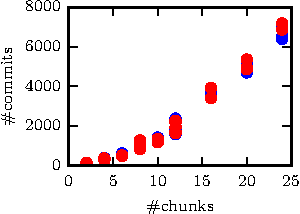
\includegraphics{floats/commits_against_project_size_for_0_fuzz_simulations}}
    \caption{Commits against project size.}
    \label{fig:no-fuzzing:features}
  \end{subfigure}
  \hfill
  \begin{subfigure}{2.3in}
    \fbox{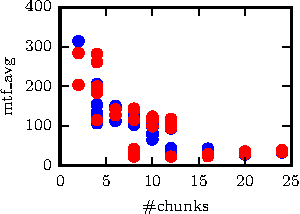
\includegraphics{floats/mtf_against_project_size_for_0_fuzz_simluations}}
    \caption{Mean time to failure.}  
    \label{fig:no-fuzzing:mtf}
  \end{subfigure}
  \hfill

  \caption{Scatter plots of software development simulations without fuzzing for Waterfall (blue) and TDD (red)
    projects.}
  \label{fig:no-fuzzing}
\end{figure}
shows that there is an exponential increase in the number of commits to the version control server as project size
increases.  This result is to be expected due to the exponential increase in the number of additional modifications,
tests, debugging and refactoring activities that would be required as a project grows in scale.  Similarly, Figure
\ref{fig:no-fuzzing:mtf} shows a decline in project quality (a reduction in the MTF from 300 to around 0 and then
stabilising for projects with more than 12 chunks) as project size increases.  Again, the additional complexity of
larger projects increases the probability of a bug causing a system failure, although MTF never declines beyond 0.
These results strengthen the claim that the model of the problem domain is plausible.


A further observation from the figures is that TDD and Waterfall workflows perform equivalently when workflows are not
subject to user distraction.  When ideal workflows are executed for both Waterfall (blue) and TDD (red), the results
show that a similar number of project commits are recorded and a similar MTF achieved.  This confirms the expectation
that the simulations of idealised workflows, whilst behaving plausibly, do not conform with expectations from the
literature that TDD should out perform waterfall.

We now proceed to compare the performance of the two software development strategies when subject to deviations in
behavior caused by distraction. Figure \ref{fig:fuzzing-features} shows scatter plots for the effect of distraction for
subsets of workflows on productivity.%
\begin{figure}[t]
  \centering
  \hfill
  \begin{subfigure}[t]{2.3in}%
    \fbox{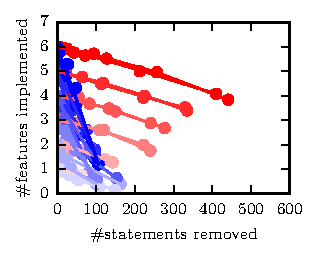
\includegraphics{floats/features_against_total_fuzz_WT}}
    \caption{Fuzzing of Waterfall and TDD.}
    \label{fig:fuzzing-features:WF}
  \end{subfigure}
  \hfill
  \begin{subfigure}[t]{2.3in}
    \fbox{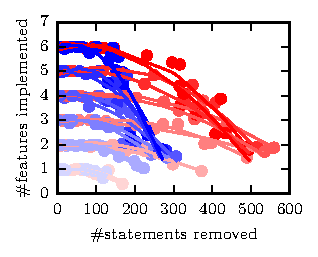
\includegraphics{floats/features_against_total_fuzz_CTIDR}}
    \caption{Fuzzing of low-level workflows.}  
  \label{fig:fuzzing-features:CTIDR}
  \end{subfigure}
  \hfill

  \caption{Scatter plots and trend lines of feature completion for Waterfall (blue) and TDD (red) for distraction
    applied to selected workflows.}
  \label{fig:fuzzing-features}
\end{figure}
In both plots, the number of features implemented for is plotted against the total number of statements removed by
fuzzing (Waterfall in blue, TDD in red). Figure \ref{fig:fuzzing-features:WF} shows the effect when only the high level
software development (Waterfall or TDD) is fuzzed, whereas Figure \ref{fig:fuzzing-features:CTIDR} shows the effect of
fuzzing lower level activities (change management, implementation, testing, debugging and refactoring). Both figures
clearly demonstrate that increasing dis- traction causes a decline in the number of completed features. However, in both
configurations, TDD is more resilient to distraction fuzzing than Waterfall, with a larger proportion of features
implemented. For fuzzing of the SDLC workflows, the decline in feature implementation appears to be highly linear, with
a far steeper decline for Waterfall than for TDD. In Figure \ref{fig:fuzzing-features}, both SDLC workflows appear to be
largely immune to distraction up to the removal of approximately 100 statements, after which feature completion
declines, with steeper declines for Waterfall.

Figure \ref{fig:fuzzing-mtf} shows the effect of distraction on MTF, again distinguishing between Waterfall (blue) and
TDD (red) SDLCs.  In these plots, both fuzzing configurations are combined, as their effects are similar.  Small and
large feature projects are plotted separately, as these have different orders of magnitude MTF.  Similar to the plots
of feature completion, the plots of MTF suggest that TDD is more resilient to fuzzing than Waterfall, which experiences
a much more dramatic decline as the number of statements removed increases.  In summary, the two comparisons of
productivity and quality demonstrate that the application of distraction fuzzing results in more realistic simulations
of user behaviour in software development workflows, as found in the available literature.
\begin{figure}[t]
  \centering
  \hfill
  \begin{subfigure}{2.3in}
    \fbox{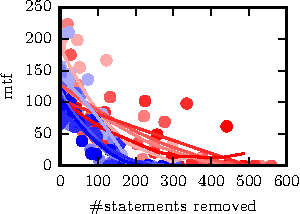
\includegraphics{floats/mtf_against_total_fuzz_projects_small}}
    \caption{Small projects.}
  \end{subfigure}
  \hfill
  \begin{subfigure}{2.3in}
    \fbox{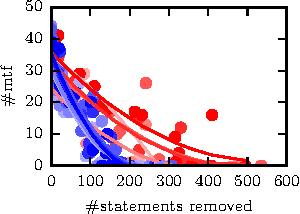
\includegraphics{floats/mtf_against_total_fuzz_projects_large}}
    \caption{Large projects.}  
  \end{subfigure}
  \hfill

  \caption{Scatter plots and trend lines of MTF for Waterfall (blue) and TDD (red) for distraction applied to all
    workflow combinations.}

  \label{fig:fuzzing-mtf}
\end{figure}

 

%%%%%%%%%%%%%%%%%%%%%%%%%%%%%%%%%%%%%%%%%%%%%%%%%%%%%%%%%%%%%%%%%%%%%%%%%%%%%%%%%%%%%%%%%%%%%%%%%%%%%%%%%%%%%%%%%%%%%%%%

\section{Conclusions}
\label{sec:conclusions}

%%%%%%%%%%%%%%%%%%%%%%%%%%%%%%%%%%%%%%%%%%%%%%%%%%%%%%%%%%%%%%%%%%%%%%%%%%%%%%%%%%%%%%%%%%%%%%%%%%%%%%%%%%%%%%%%%%%%%%%%

This paper has presented and evaluated a novel approach to modelling and simulating realistic user behaviours when
interacting with information systems, through the use of model fuzzing aspects.  The novelty of this appraoch is the
ability to model the causes of realistic user behaviour (such as distraction) separately as aspects that can
subsequently applied flexibly to many different workflows in a simulation. The efficacy of the approach is demonstrated
in a by showing that the introduction of realistic user behaviour into simulations of software development workflows
gives results that better conform with empirical evidence available in the literature.

The proof of concept presents the opportunity for a substantial research agenda in the modelling and simulation of user
interaction with information systems, in order to better predict emergent socio-technical system properties. Further
research is necessary to test the viability of the approach when applied to larger, more complex scale socio-technical
systems, such as the election e-counting system described by \citet{lock07observations}, comprising whole information
infrastructures and hundreds or thousands of diverse users.  This will provide opportunities to experiment with a
variety of other causes of variability in socio-technical system behavior, such as subjective misjudgments, exhaustion,
misordering of steps and shortcut taking.  Further interdisciplinary research is required to develop and validate the
realism of socio-technical fuzzing aspects that implement these behaviors. There is a need to link empirical evidence of
the causes and occurrence of these behaviors to their impact on the operation of workflows.  The overall aim of this
research agenda is towards simulation techniques that can have predictive capabilities suitable for informing systems
engineering decisions before resources are committed to construction.  The availability of such tools would do much to
progress the current craft of large scale socio-technical systems engineering.


%%%%%%%%%%%%%%%%%%%%%%%%%%%%%%%%%%%%%%%%%%%%%%%%%%%%%%%%%%%%%%%%%%%%%%%%%%%%%%%%%%%%%%%%%%%%%%%%%%%%%%%%%%%%%%%%%%%%%%%% 

\bibliographystyle{splncsnat}

\bibliography{references,repositories}

%%%%%%%%%%%%%%%%%%%%%%%%%%%%%%%%%%%%%%%%%%%%%%%%%%%%%%%%%%%%%%%%%%%%%%%%%%%%%%%%%%%%%%%%%%%%%%%%%%%%%%%%%%%%%%%%%%%%%%%%





\end{document}
